\chapter{Computational Homology}

Homology is one way of analyzing \textit{local} properties in order to extract information about \textit{global} phenomenon. As large amounts of data become available, it becomes more difficult to determine what information is relevant. There are, of course, high and low-level approaches. A high-level approach like a fingerprint scanner or handwriting recognition might be the end-goal of one's analysis, but lower-level approaches like homology look at the geometric makeup of an object and is often a requisite step toward building higher-level processes.

	At this time, computational homology is a relatively new field and its application in physics has only recently been explored. Although homology is a field of algebraic topology, it combines the mathematics of several other fields including combinatorics and computation. The mathematical formalism behind homology is difficult to grasp so only the relevant information will be detailed here.
	
\section{Image analysis}

To put it simply, homology is concerned with \textit{holes} and \textit{pieces}. Mathematically, how does one define a ``hole''? What does it mean to be part of a ``connected piece''? It's best to think about this in one dimension first. \refFig{fig:homology1d} shows two simple topological spaces, $X$ and $Y$. Although $X$ and $Y$ are spaces with one and two line segments respectively, in terms of homology one would say $X$ consists of a single \textit{connected piece} while $Y$ has two distinct pieces. The fact that the line segments are straight or of different length is not important for the homology. In this one-dimensional example, the \textit{zeroth homology groups} of each are

\begin{align}
	& H_0(X) \cong \mathbf{Z}^1  & \text{and} & \quad H_0(Y) \cong \mathbf{Z}^2
	\label{eq:homology1d}
\end{align}

where $\mathbf{Z}$ is the group of integers. The homology pairs a topological space (e.g.\ $X$ and $Y$) with an \textit{abelian group}, a set of elements combined with operations that satisfy five axioms (closure, associativity, identity, invertibility, and commutativity). Notice, however, that the \textit{zeroth homology grou}p of $Y$ is $\mathbf{Z}^2$; the exponent, $2$, is what accounts for the two ($2$) distinct pieces, but more on this later.

\begin{figure}
	\begin{center}
		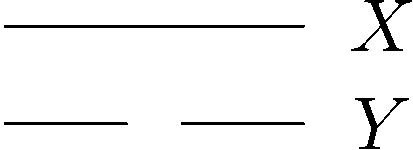
\includegraphics[width=0.2\columnwidth]{Figs/homology1d.pdf}
		\caption{\label{fig:homology1d} Topological spaces $X$ and $Y$. $X$ consists of one connected line segment and $Y$ has two disconnected line segments.}
	\end{center}
\end{figure}

Since there is a \textit{zeroth homology group}, it makes sense that there would be a \textit{first homology group}. Looking at the two-dimensional example in \refFig{fig:homology2d}, the homology of each space $X_a$, $X_b$, $X_c$, and $X_d$ is

\begin{align}
	H_1(X_a) \cong 0  & \quad H_1(X_b) \cong \mathbf{Z} & \quad H_1(X_c) \cong 0 & \quad H_1(X_d) \cong \mathbf{Z} \\
	H_0(X_i) \cong \mathbf{Z} & \qquad \text{for} & \quad i = a, b, c, d \label{eq:homology2d}
\end{align}

\begin{figure}
	\begin{center}
		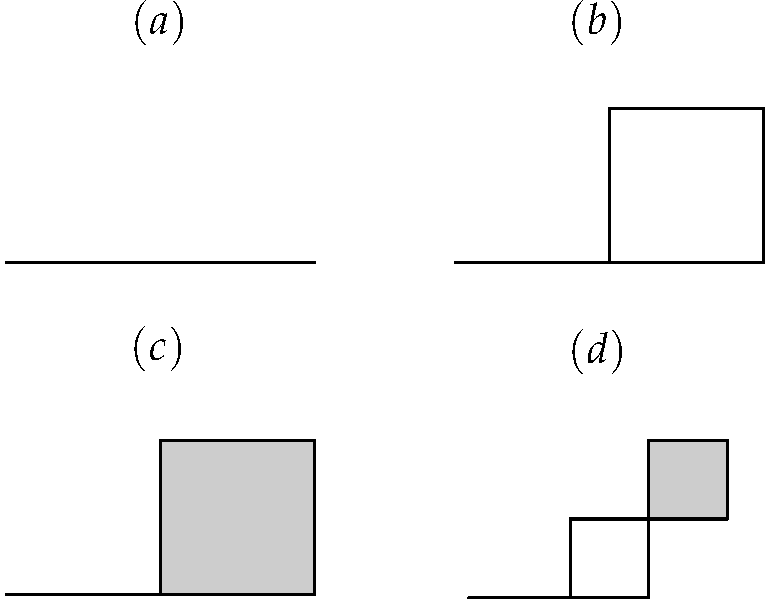
\includegraphics[width=0.6\columnwidth]{Figs/homology2d.pdf}
		\caption{\label{fig:homology2d} Topological spaces $X_a$, $X_b$, $X_c$, and $X_d$.}
	\end{center}
\end{figure}

All spaces $X_i$ for $i = a,b,c,d$ have a \textit{zeroth homology group} of $\mathbf{Z}$ since there is a single connected component. In \refFig{fig:homology2d}(b)-(c), the connected component forms an enclosed area (\eg the squares). The square in (b) forms a ``hole''. The shading indicates that the hole is filled and is thus no longer a ``hole''. \refFig{eq:homology2d}(b), (d) both contain one hole while (a), (c) contain zero holes. Just as the \textit{zeroth homology group} is concerned with connected segments, the \textit{first homology group} is concerned with ``holes''.

The terms ``piece'' and ``hole'' are informal. Formally, we could say that the $k^{th}$ homology group, $H_k(X)$, represents the $k$-dimensional \textit{holes} of $X$ where a 0-dimensional \textit{hole} is merely the gap between two components (\eg $Y$ in \reffig{eq:homology1d}).


